% =============================================================================
% IT-Innovation -- A3-Poster zur Masterarbeit (ALTERNATIVES DESIGN)
% Identischer Inhalt wie poster_a3.tex, aber Karten-/Box-Layout statt Linien.
% Kompilieren:  pdflatex poster_a3_cards.tex
% Bilder werden aus ../thesis/images/ gezogen (siehe \graphicspath).
% =============================================================================
\documentclass[10pt]{scrartcl}

\usepackage[utf8]{inputenc}
\usepackage[T1]{fontenc}
\usepackage[ngerman]{babel}
\usepackage{lmodern}
\usepackage[a3paper,landscape,margin=1.2cm]{geometry}
\usepackage{graphicx}
\usepackage[table]{xcolor}
\usepackage{multicol}
\usepackage{booktabs}
\usepackage{tabularx}
\usepackage{enumitem}
\usepackage{microtype}
\usepackage[most]{tcolorbox}
\usetikzlibrary{arrows.meta}

\graphicspath{{../../thesis/images/}{../}}

% --- Farbpalette (anpassbar) -------------------------------------------------
\definecolor{primary}{RGB}{0,95,115}    % Petrol/Teal
\definecolor{accent}{RGB}{202,103,2}     % Amber/Orange
\definecolor{cardbg}{RGB}{247,250,251}   % sehr helles Grau-Blau
\definecolor{cardbgA}{RGB}{253,247,240}  % sehr helles Amber-Tint
\definecolor{ink}{RGB}{33,42,46}

% --- Layout ------------------------------------------------------------------
\setlength{\columnsep}{0.9cm}
\setlength{\parindent}{0pt}
\setlength{\parskip}{0.30em}
\color{ink}
\pagestyle{empty}

% Karten-Stil (Petrol) -- farbiger Titelbalken, gerahmter heller Body
\newtcolorbox{pbox}[1]{%
  enhanced, breakable=false,
  colback=cardbg, colframe=primary, boxrule=0.9pt,
  colbacktitle=primary, coltitle=white,
  fonttitle=\bfseries\large, title={#1},
  arc=1.4mm, boxsep=1.2mm, left=2.4mm, right=2.4mm, top=1.4mm, bottom=1.6mm,
  before skip=2pt, after skip=8pt,
  attach boxed title to top left={xshift=2mm, yshift=-2.4mm},
  boxed title style={arc=1mm, boxrule=0pt},
  top=4mm}

% Karten-Stil (Amber) -- Akzentvariante
\newtcolorbox{pboxA}[1]{%
  enhanced, breakable=false,
  colback=cardbgA, colframe=accent, boxrule=0.9pt,
  colbacktitle=accent, coltitle=white,
  fonttitle=\bfseries\large, title={#1},
  arc=1.4mm, boxsep=1.2mm, left=2.4mm, right=2.4mm, top=1.4mm, bottom=1.6mm,
  before skip=2pt, after skip=8pt,
  attach boxed title to top left={xshift=2mm, yshift=-2.4mm},
  boxed title style={arc=1mm, boxrule=0pt},
  top=4mm}

% Bild + kleine Unterschrift (multicol-tauglich)
\newcommand{\posterfig}[3]{% #1 = datei, #2 = breite (0..1), #3 = caption
  \par\nobreak\vspace{0.25em}%
  \noindent\begin{minipage}{\linewidth}\centering
    \includegraphics[width=#2\linewidth]{#1}\\[0.2em]
    {\footnotesize\itshape #3}%
  \end{minipage}\par\vspace{0.15em}}

\begin{document}

% --- Kopfbereich: dunkles Hero-Band -----------------------------------------
\begin{tcolorbox}[colback=primary, colframe=primary, arc=3mm, boxrule=0pt,
  left=6mm, right=6mm, top=3.5mm, bottom=3.5mm, enhanced,
  borderline west={5mm}{0mm}{accent}]
\begin{minipage}[c]{0.78\textwidth}
  \color{white}
  {\Huge\bfseries Prognose individuellen Mobilitätsverhaltens}\\[0.3em]
  {\LARGE auf Basis eines mit Bewegungsdaten trainierten Machine-Learning-Modells}\\[0.6em]
  {\newline\large Achim Baumgärtner
   \quad\textbar\quad Betreuung: Gian Ledl-Truöl, Prof.\,Dr.\ Sonntag
   \quad\textbar\quad Fakultät Informatik und Informationstechnik, Hochschule Esslingen
   \newline\newline\textbf{AIM Angewandte Informatik}}
\end{minipage}\hfill
\begin{minipage}[c]{0.20\textwidth}
  \begin{tcolorbox}[colback=white, colframe=white, arc=2mm, boxrule=0pt,
    halign=center, valign=center, left=2mm, right=2mm, top=2mm, bottom=2mm]
    
\includegraphics[height=2.0cm]{HochschuleEsslingen_Logo_4c_DE.png}\\[0.5em]
    
\includegraphics[height=1.3cm]{KEIM-quadr.png}
  \end{tcolorbox}
\end{minipage}
\end{tcolorbox}

\vspace{0.4em}

% --- Drei Spalten ------------------------------------------------------------
\begin{multicols}{3}
\raggedcolumns

\begin{pbox}{Motivation}
Der wachsende Anteil erneuerbarer Energien erzeugt ein Speicherproblem:
überschüssiger Strom lässt sich bislang kaum wirtschaftlich speichern.
\textbf{Elektrofahrzeuge} können als mobile, verteilte Speicher dienen und
über \emph{Vehicle-to-Grid} (V2G) Energie ins Netz zurückspeisen. Voraussetzung
ist, dass bekannt ist, \emph{wann} ein Fahrzeug genutzt wird und wann es dem Netz zur Verfügung steht -- eine Fehleinschätzung kann bis zur Nichtverfügbarkeit des Fahrzeugs führen.

\vspace{0.4em}
\begin{center}
\resizebox{0.98\linewidth}{!}{%
\begin{tikzpicture}[>={Stealth[length=2.4mm]}, font=\footnotesize]
  % erneuerbare Energie (Photovoltaik)
  \node[inner sep=0pt] at (0,0) {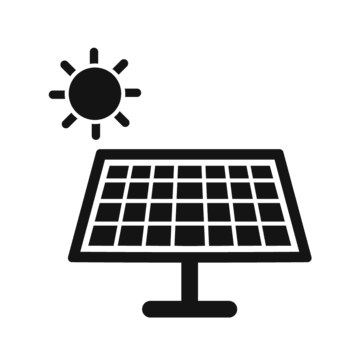
\includegraphics[width=1.6cm]{pv.png}};
  \node[align=center] at (0,-1.05) {erneuerbare\\Energien [8]};
  % Stromnetz
  \node[draw=primary, line width=1pt, rounded corners=1mm, fill=white,
        minimum width=1.7cm, minimum height=1.05cm, align=center] (grid) at (3,0)
        {Strom-\\netz};
  % E-Fahrzeug
  \begin{scope}[shift={(6.2,-0.16)}]
    \fill[primary] (-0.64,0) rectangle (0.64,0.34);
    \fill[primary] (-0.36,0.34) -- (-0.18,0.62) -- (0.32,0.62) -- (0.48,0.34) -- cycle;
    \fill[ink] (-0.36,0) circle (0.13);
    \fill[ink] (0.38,0) circle (0.13);
    \node[white] at (0.03,0.17) {\scriptsize\bfseries EV};
  \end{scope}
  \node[align=center] at (6.2,-1.05) {Elektro-\\fahrzeug};
  % Pfeile
  \draw[->, line width=1.2pt] (0.82,0) -- (grid.west)
        node[midway, above, align=center]{};
  \draw[<->, line width=1.2pt, accent] (grid.east) -- (5.5,0)
        node[midway, above]{\textbf{V2G}};
  % Aufhaenger: Prognosefrage
  % Analoge Uhr als Aufhaenger (wann ist das Fahrzeug verfuegbar?)
  \begin{scope}[shift={(6.2,1.25)}]
    \draw[primary, line width=1pt] (0,0) circle (0.32);
    \foreach \a in {0,30,...,330}{\draw[primary, line width=0.5pt] (\a:0.27) -- (\a:0.32);}
    \draw[primary, line width=1.1pt] (0,0) -- (75:0.15);
    \draw[primary, line width=1.1pt] (0,0) -- (90:0.24);
    \fill[primary] (0,0) circle (0.03);
    \node[primary] at (0.62,0) {\large\bfseries ?};
  \end{scope}
  \draw[->, primary, dashed, line width=0.9pt] (6.2,0.88) -- (6.2,0.52);
\end{tikzpicture}}
\end{center}
\end{pbox}

\begin{pboxA}{Problem \& Forschungslücke}
Bestehende Arbeiten behandeln überwiegend das \emph{Lade}verhalten oder
\emph{aggregierte} Gruppen. Das \textbf{individuelle} Fahrverhalten einzelner
Fahrzeuge wird kaum modelliert, obwohl es stark heterogen ist~[1]. Zudem fehlt ein einheitliches Datenformat: Datensätze unterscheiden sich erheblich in Schema, Auflösung und Qualität.
\end{pboxA}

\begin{pbox}{Forschungsfragen}
\begin{enumerate}[leftmargin=1.3em,itemsep=0.15em,topsep=0.1em]
  \item Wie zuverlässig lässt sich individuelles Mobilitätsverhalten über bis
        zu sieben Tage vorhersagen, und wie unterscheiden sich die Lernverfahren?
        Welchen Einfluss hat die \textbf{Datenqualität} -- getrennt vom \textbf{Algorithmus}?
  \item Welche Anforderungen an die Datengrundlage ergeben sich, und wie lässt sich ihre Qualität bewerten?
\end{enumerate}
\end{pbox}

\begin{pboxA}{Ziele}
\begin{itemize}[leftmargin=1.2em,itemsep=0.12em,topsep=0.1em]
  \item ein zuverlässiges Prognosemodell für das individuelle Mobilitätsverhalten (1--7 Tage),
  \item Vergleich mehrerer Lernverfahren hinsichtlich Genauigkeit,
  \item Trennung des Daten- vom Algorithmus-Effekt,
  \item kalibrierte Unsicherheit (P10/P90) als Entscheidungsgrundlage für die Netzsteuerung.
\end{itemize}
\end{pboxA}

\begin{pbox}{Daten}
In Ihrem ursprünglichen Format waren die Daten nicht zu verwerten und mussten daher einheitlich verarbeitet werden. Im Moment werden fünf heterogene Quellen werden über einen Adapter auf ein einheitliches Schema (\texttt{vehicle\_id, timestamp, driving}) gebracht:

\vspace{0.2em}
{\footnotesize
\begin{tabularx}{\linewidth}{@{}lX@{}}
\toprule
\textbf{Quelle} & \textbf{Charakter} \\
\midrule
emobpy        & synthetische BEV-Profile~[2] \\
real\_world\_ev & reale EV-Felddaten~[3] \\
VED           & Fahrzeug-Energiedaten~[4] \\
routine       & regelbasierte Referenz \\
YJMob100K     & menschl.\ Bewegungsdaten (Kontrast)~[5] \\
\bottomrule
\end{tabularx}}

\posterfig{data_emobpy.png}{0.5}{heterogene Rohdatenform (emobpy)}
\end{pbox}

\begin{pboxA}{Methodik}
Zwei überwachte Teilaufgaben: \textbf{Klassifikation} (fährt vs.\ geparkt, pro Stunde) und \textbf{Regression} (Abfahrts-/Rückkehrzeit). Aus den Rohdaten werden Kalender-, Lag- und Rolling-Merkmale abgeleitet; Lags respektieren die Fahrzeuggrenzen (kein Datenleck).

\posterfig{prozess_diagrammred.png}{0.62}{Verarbeitungs-Pipeline der Mobilitätsdaten}

Als Verfahren dienen baumbasierte Ensembles -- \textbf{Random Forest}~[6] als Baseline und \textbf{Gradient Boosting (LightGBM)}. Beide liefern Unsicherheits- bänder (P10/P90); ein autoregressives Monte-Carlo-Rollout erzeugt stundengenaue Prognosen. Das starke Klassenungleichgewicht (Fahrzeuge stehen meist) wird durch \textbf{Klassengewichtung} ausgeglichen.

\posterfig{decisiontree2red.png}{0.34}{Entscheidungsbaum: Split nach Gini-Unreinheit}
\end{pboxA}

\begin{pbox}{Evaluationsdesign \& Ergebnis}
Eine \textbf{Kreuzvalidierungs-Matrix} trainiert je Modell auf einer Quelle und testet auf \emph{allen}. Da Algorithmus und Merkmale konstant bleiben, isoliert sie den \textbf{Daten-} vom \textbf{Algorithmus-Effekt}. Alle Splits sind \textbf{zeitlich} (Vergangenheit\,$\rightarrow$\,Training, Zukunft\,$\rightarrow$\,Test), nie zufällig.

\posterfig{cv_f1_5x5blue.png}{0.6}{F1 der 5$\times$5-Kreuzvalidierung}

Die Diagonale (In-Domain) ist meist am stärksten. \texttt{VED} bleibt schwach (nur Fahrt-Logs, rekonstruierte Parkzeiten), während leicht prognostizierbare Quellen mit hoher Aktiv-Rate (\texttt{routine}, \texttt{YJMob}) hohe Werte erreichen -- der \textbf{Einfluss der Datenquelle} wird klar sichtbar.
\end{pbox}

\begin{pboxA}{Fazit \& Ausblick}
Die Arbeit schafft die Grundlage für eine fahrzeugbasierte, vorausschauende Steuerung von Energieflüssen. Da menschliche Mobilität eine prinzipielle Vorhersagbarkeitsgrenze besitzt~[7], steht nicht die perfekte Prognose im Fokus, sondern \textbf{belastbare, unsicherheitsbewusste} Aussagen. Ausblick: sequenzielle Modelle (LSTM, Transformer) und \"Ubertragbarkeit auf neue Nutzer.
\end{pboxA}

\begin{pbox}{Quellen}
{\footnotesize\setlength{\parskip}{0.15em}
[1]~Ji et al., \emph{Rethinking the Regularity in Mobility Patterns}, T.\ in GIS, 2023.\par
[2]~Gaete-Morales et al., \emph{emobpy}, Zenodo, 2020.\par
[3]~Pozzato et al., \emph{Real-World EV Field Data}, Mendeley, 2023.\par
[4]~Oh et al., \emph{Vehicle Energy Dataset (VED)}, IEEE T-ITS, 2022.\par
[5]~Yabe et al., \emph{YJMob100K}, Scientific Data, 2024.\par
[6]~Breiman, \emph{Random Forests}, Machine Learning, 2001.\par
[7]~Song et al., \emph{Limits of Predictability in Human Mobility}, Science, 2010.\par
[8]~PV-Icon: \emph{Cartoon Solar Panels}, Pngtree, \newline \texttt{pngtree.com/freepng/cartoon-solar-panels\_2067893.html}\par}
\end{pbox}

\end{multicols}
\end{document}
